% Please use the skeleton file you have received in the 
% invitation-to-submit email, where your data are already
% filled in. Otherwise please make sure you insert your 
% data according to the instructions in PoSauthmanual.pdf

% JRP added to avoid ifpdf name clash in TexShop
\RequirePackage{ifpdf}
%%% END JRP

\documentclass{PoS}

%JRP added
%Uncomment next line if AMS fonts required
 \usepackage{graphicx}
 \usepackage{epstopdf}
 %%% END JRP

\title{Synergy with CO/[CII] Line Intensity Mapping}

\ShortTitle{CO/[CII] synergy}

\author{\speaker{Chang}\thanks{A footnote may follow.}, Aguirre, Gong,
  Pritchard,  on behalf of the EoR/CD-SWG\\
        ASIAA\\
        E-mail: \email{tcchang@asiaa.sinica.edu.tw}}

%\author{Another Author\\
%        Affiliation\\
%        E-mail: \email{...}}

\abstract{

This subchapter will describe cross-correlation sciences and synergy
with the SKA1-low 21-cm EoR surveys enabled by other programs, in particular
promising line intensity mapping surveys of CO rotational lines, [CII] and Ly-$\alpha$ emissions during
reionization are discussed.

}

\FullConference{
Advancing Astrophysics with the Square Kilometre Array\\
June 8-13, 2014\\
Giardini Naxos, Italy}

%Add new definitions here
%user defined shortcuts
%Journal definitions
\newcommand{\apj}{ApJ}
\newcommand{\apjl}{ApJ}
\newcommand{\apjs}{ApJS}
\newcommand{\aap}{A \& A}
\newcommand{\aj}{AJ}
\newcommand{\araa}{ARAA}
\newcommand{\mnras}{MNRAS}
\newcommand{\physrep}{Phys. Rep.}
\newcommand{\prd}{PRD}
\newcommand{\nat}{Nat.}
\newcommand{\jcap}{JCAP}
\newcommand{\sovast}{Sov. Astron.}
\newcommand{\nar}{New Astron. Rev.}
\newcommand{\apss}{Astrophys. \& Space. Sci.}

%%%% END NEW DEFINITIONS

\begin{document}

%%%%%%%%%%%%%%%%%%%%%%%%%%%%%
%%%%%%%%%%%%%%%%%%%%%%%%%%%%%
\section{Introduction}

While the distribution of neutral
hydrogen mapped by SKA1-low provides an excellent and unique view of the reionization
process over a large range of redshifts, detecting sources responsible for
reionization directly sheds light on the crucial stage of galaxy
formation and complements our understanding of EoR.   Extremely deep
imaging with the Hubble Space Telescope (HST) has begun to probe the very bright end of the UV
luminosity functions at z > 6 \cite{2014arXiv1403.4295B, 2013ApJ...768...71R}, with improvements expected 
with the  James Webb Space Telescope (JWST). In the sub-mm, ALMA has
detected individual high redshift, luminous objects known from
existing surveys (e.g., \cite{2013ApJ...778..102O}). However, observations that are aimed at
detecting individual galaxies at z > 6 are difficult and time
consuming, and neither of these space-borne facilities nor ALMA is
expected to resolve the majority of sources responsible for
reionization at z > 8 \cite{2011MNRAS.414..847S}.  Approaches which can access the entire
luminosity function of reionizing sources are needed.

Line Intensity Mapping has emerged as a promising technique that is sensitive
to the integrated light produced by faint galaxies: instead of
resolving individual sources, one measures on larger spatial scales the collective emission
from an ensemble of sources, while retaining the spectral thus redshift
information.  This allows efficient redshift surveys that probe the
integrated luminosity function of sources and provide three-dimensional
information to study star formation activities at EoR. 

\begin{figure}[htbp]
\begin{center}
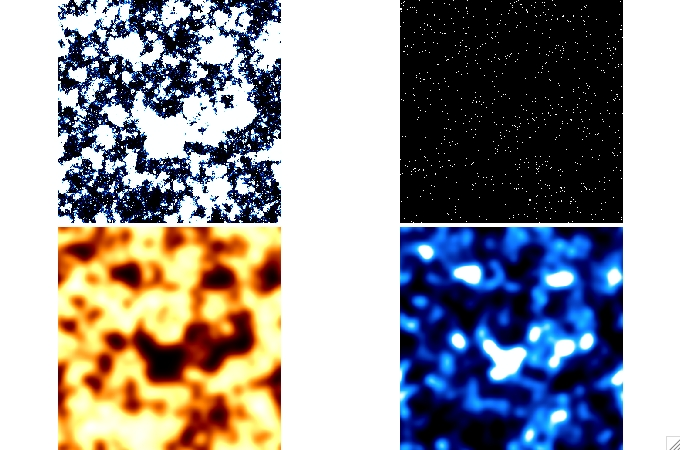
\includegraphics[scale=0.35]{figures/21cm_co_ion_gal_b.jpg}
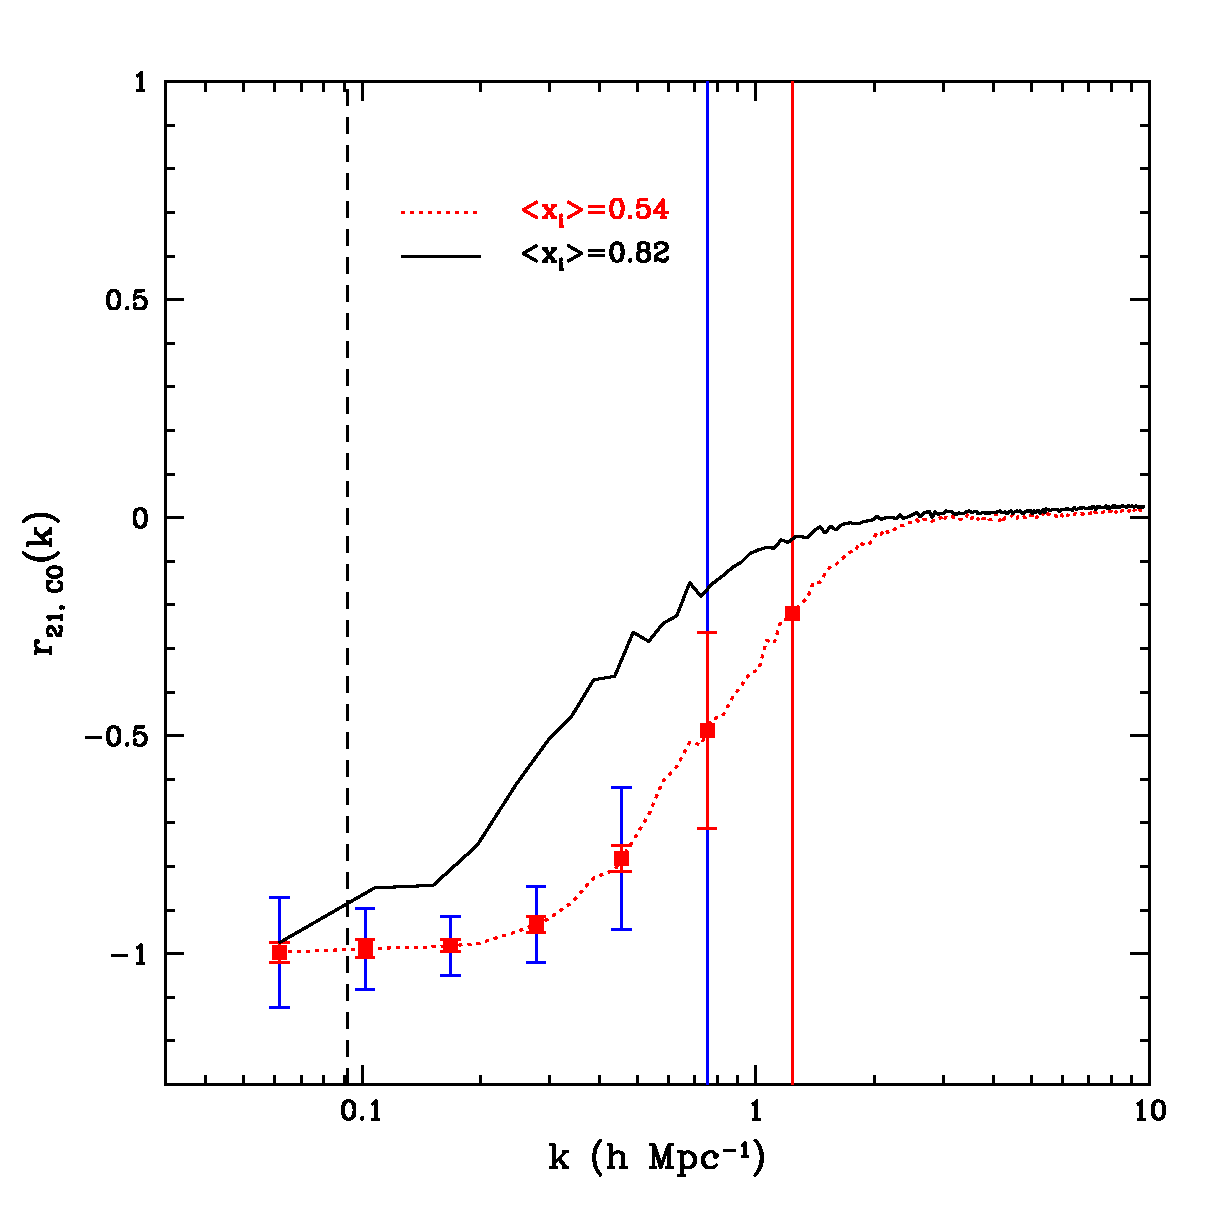
\includegraphics[scale=0.3]{figures/co_21cm_cross_col.eps}
\caption{{\em Left panel: } 21cm, CO, galaxy, and ionisation fields \cite{2012RPPh...75h6901P}. {\em Right panel: } Cross-correlation between CO and 21cm signal \cite{2011ApJ...741...70L}.}
\label{fig:cross_col}
\end{center}
\end{figure}
Figure \ref{fig:cross_col} illustrates the utility of an intensity mapping survey. Molecular gas is associated with the galaxies that produce ionisation photons leading to an anti-correlation between the 21cm signal and the CO signal. This anti-correlation is potentially detectable and gives a clear indication of the size of ionised regions \cite{2011ApJ...741...70L}. Simultaneous detection of the intensity mapping signal from galaxies responsible for ionising photons and 21cm detection of the remnant neutral hydrogen would provide a powerful constraint on process of reionization.

%%%%%%%%%%%%%%%%%%%%%%%%%%%%%
%%%%%%%%%%%%%%%%%%%%%%%%%%%%%
\section{CO}


%%%%%%%%%%%%%%%%%%%%%%%%%%%%%
%%%%%%%%%%%%%%%%%%%%%%%%%%%%%
\section{CII}

%%%%%%%%%%%%%%%%%%%%%%%%%%%%%
%%%%%%%%%%%%%%%%%%%%%%%%%%%%%

\section{Ly-$\alpha$}


%%%%%%%%%%%%%%%%%%%%%%%%%%%%%
%%%%%%%%%%%%%%%%%%%%%%%%%%%%%
\section{Paths to Phase 2}

%%%%%%%%%%%%%%%%%%%%%%%%%%%%%
%%%%%%%%%%%%%%%%%%%%%%%%%%%%%
\section{Summary}

%%%%%%%%%%%%%%%%%%%%%%%%%%%%%
%%%%%%%%%%%%%%%%%%%%%%%%%%%%%


\bibliographystyle{unsrt}
\bibliography{synergy}{}

\end{document}
